\section{Dataset}
We finally obtained a relatively large-scale timestamp-aligned dataset of \texttt{<word, location, activity>}, with various context and sound types, details provided as follows. 

\subsection{Statistics of the dataset}
%\KZ{Because one of the contributions of this paper is the dataset,
	%you should give the stats of the raw videos, number of words segmented out,
	%and then the distributions of the word types, activities and locations, etc.
	%Give a table here.}
The dataset contains 8,926 triplets from corresponding 3,390 videos and 5186 sentences, including 6 different types of dog sound, 11 location categories, and 12 activity categories as shown in ~\tabref{tab:dataset}. The types of words are defined in AudioSet and we list out the most frequent scenes and activities tailored for Shiba Inu by combining commonsense and data manual checking for location and activity. We have an average of 1.7 words in a sentence and 1.5 sentences in a video. Some basic statistics of the dataset can be seen in ~\tabref{tab:datainformation1}.
%\MY{This sounds amateur, try saying that we listed out the most frequent scenes and activities tailored for Shiba Inu by combining commonsense and data manual checking. e.g. u get information from the subtitles, raw results of pretrained model etc.}. 
%\MY{how? if this sentence is talking about 4.2, then leave everything there}.
%The average, max, min length of a word is respectively 0.8 seconds, 3 and 0.08 seconds. We have averagely 1.7 words in a sentence and 1.5 sentences in a video.  
%\KZ{The filering should have been talked about in approach.}

\begin{table}[th]
	\small
	\begin{tabular}{p{0.14\columnwidth}|p{0.8\columnwidth}}
		\toprule
		\textbf{Context} & \textbf{Possible values} \\ \midrule
		Word & Bow-wow, Bark, Whimper, Growl, Howl, Yip \\ \midrule
		Location & Living room, Food nearby, Grass, Cage, Road, Bathroom, Snowfield, Beach, Square, Cabin, Others    \\ \midrule
		Activity & Laying down, Playing with human, Standing, Sitting, Walking, Begging for food, PLaying with a toy, Taking a shower, Running, Eating, Sniffing, Unknown \\ 
		\bottomrule
	\end{tabular}
	\caption{Respective categories in the triplet.}
	%\KZ{Change ``growling'' to growl everywhere incl.
		%the figures to be consistent, since yip, growl, howl, etc. are both verbs and nouns.}}
%\KZ{How did we define the domains of these values?
	%Please give citations and sources.}}
	\label{tab:dataset}
\end{table}

~\figref{fig:distri} shows the prior distribution of our data across different sound types, location types, and activity types. This data imbalance reflects real-world data distribution, that pet dogs kept at home are more prone to stay in the living room and exhibit activities like laying down and playing with humans.
%\MY{consider saying: this data imbalance reflects real-world data distribution, that pet dogs kept at home are more prone to stay in living room and exhibit activities like laying down and playing with human}. 
We take this imbalanced prior distribution into consideration when computing the correlations between them. 
%\MY{awkward sentence, just say that we take this imbalanced prior distribution into consideration when computing the correlations between them}.
%\KZ{Add a figure/table to show the stats of the words/sentences that we got,
%like the avg len, min/max len, variance, how many words per sentence, how many
%words per video, etc. These will be interesting stats to show the scale and
%significance of our dataset.}

\begin{table}[th]
	\small
	\centering
	\begin{tabular}{p{0.2\columnwidth}|p{0.15\columnwidth}|p{0.15\columnwidth}|p{0.15\columnwidth}}
		\toprule
		& Min len & Max len & Avg. len \\ \midrule
		Bow-wow & 0.16s & 2.88s & 0.51s  \\ \midrule
		Yip & 0.16s & 2.92s & 0.60s\\ \midrule
		Whimper & 0.16s & 2.76s & 0.62s\\ \midrule
		Bark & 0.20s & 2.88s& 0.67s \\ \midrule
		Growl & 0.20s & 2.96s & 0.79s\\ \midrule
		Howl & 0.16s & 2.96s & 0.98s\\
		\bottomrule
	\end{tabular}
	\caption{Statistics of dataset. The columns are respectively the minimum, maximum and average length of a word.}
	\label{tab:datainformation1}
\end{table}








\begin{figure*}[ht]
\centering
%\subfigure[Word type distribution]{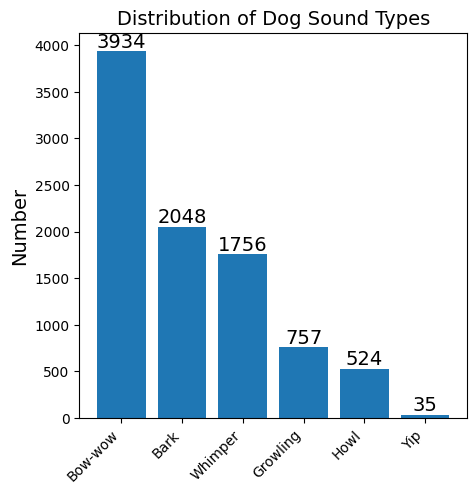
\includegraphics[width=0.32\hsize, height=0.28\hsize]{images/sound_distri.png}}
%\subfigure[Location type distribution]{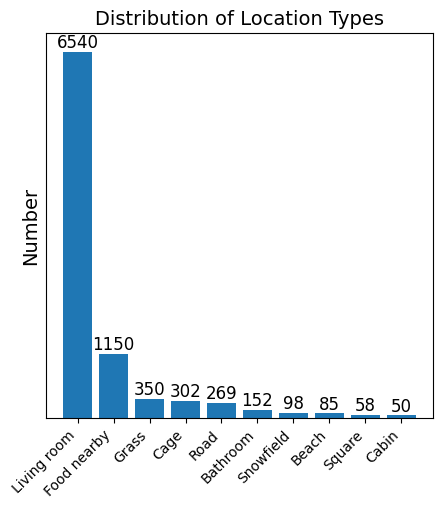
\includegraphics[width=0.32\hsize, height=0.28\hsize]{images/location_distri.png}}
%\subfigure[Activity type distribution]{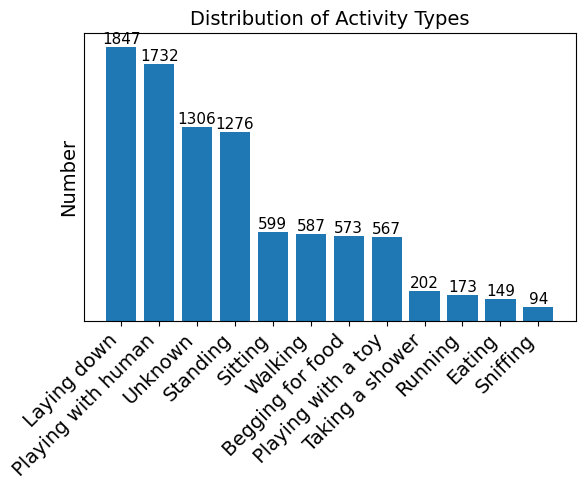
\includegraphics[width=0.32\hsize, height=0.28\hsize]{images/activity_distri.png}}
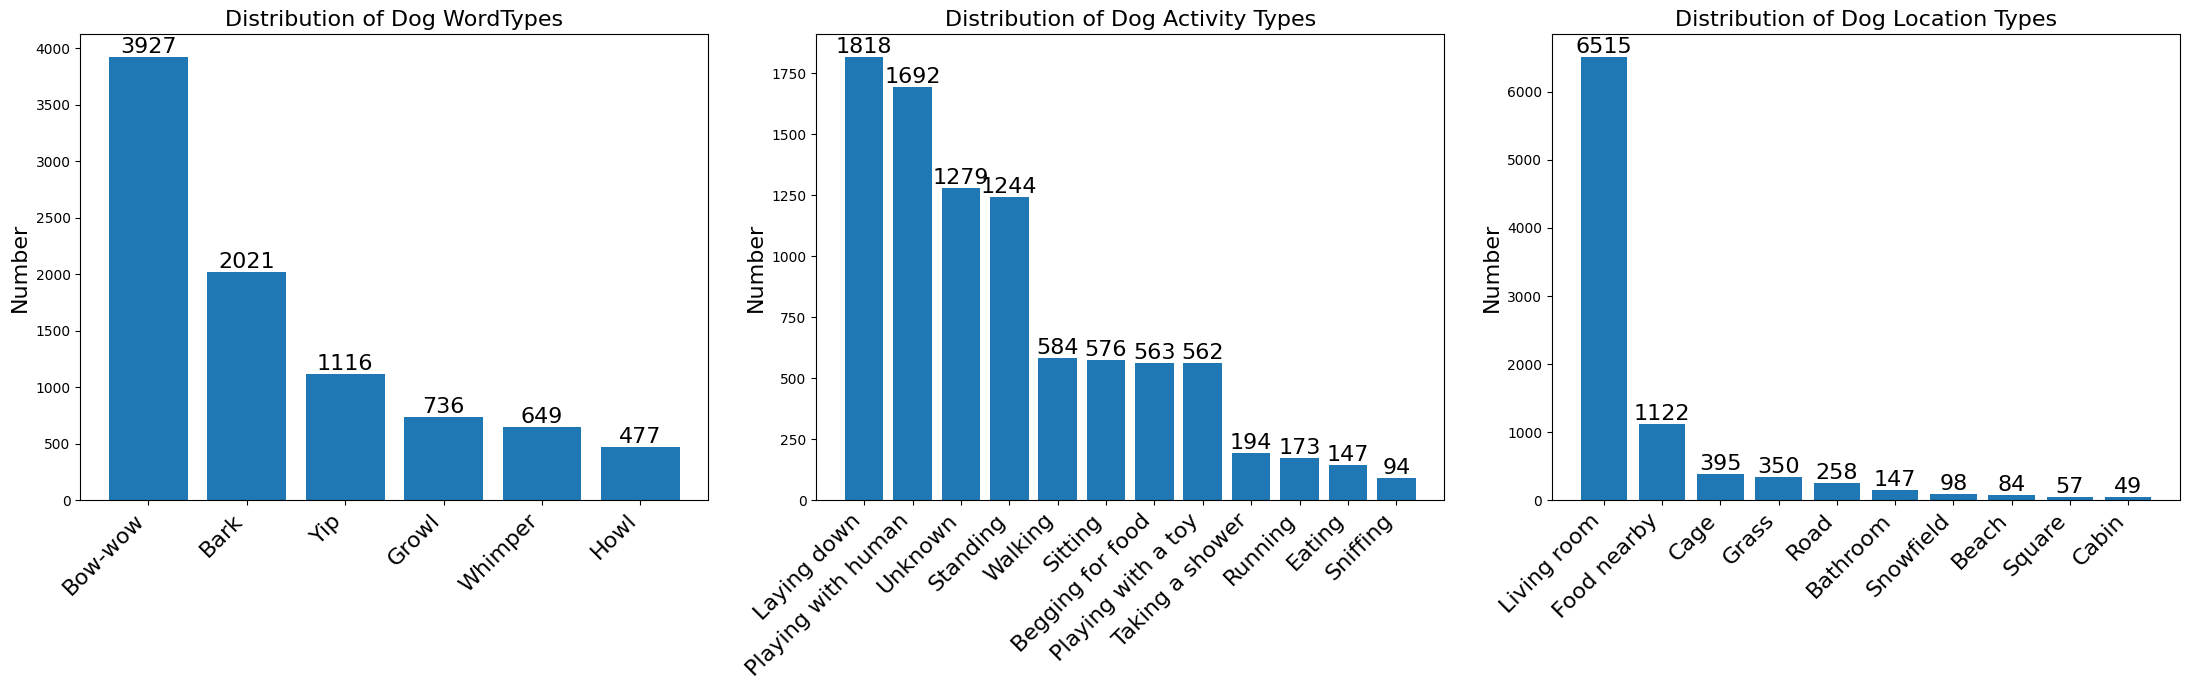
\includegraphics[width=1.99\columnwidth]{images/data_distri.png}
\caption{Prior distributions of word types, locations and activities in
the triple sequences. The numbers shown are the number of triplets \texttt{<word, location, activity>}
with a particular word, location, or activity.} %\KZ{Change growling to growl.}} %\KZ{Make these three plots equal size.} \AT{will be modified after having whimper yip result}} 
%\KZ{Always
%add full stop at the end of each caption. Pls make the words on the x-axis slanted a bit (just like (a) to save space. Pls do that for the rest of the figs.
%Why is the Yip so little? In my experience, I hear this kind of sound quite 
%often in the dogs. The distribution is too skewed. Is it possible
%that the recall of Yip is not good enough? Can we present a confusion
%matrix among these 6 types from the classification results?}}
\label{fig:distri}
\end{figure*}

\subsection{Quality of the triples}
%\KZ{Give the acc numbers of each steps in \figref{fig:method}.}
%\KZ{You need to give details on how you acheive these accuracy numbers.
%Like how u sampled, how many judges, how to judge, etc.}
We present the accuracy of each step to ensure the high quality of our dataset. For word segmentation and word classification, we randomly sample 200 segmented
words to listen to. Three annotators have to label whether this is a singular
dog word and whether the word is correctly classified. 
Their respective accuracy is 0.95 and 0.73.
We achieve an accuracy of 0.78 for location classification on our manually labeled pictures and an accuracy of 0.59 for the top 1 and 0.9416 for the top 5 for activity classification.

\section{Results and Analysis}
\label{sec:results}
%\KZ{Rephrase this para:
In this section, we present our analysis of the data. We analyze uni-gram and bi-gram relationships with words and context. Then we present a summarization of findings that uncovers dog vocalization patterns. 
\subsection{Analysis of word type and location}
The vocalization of a dog may vary depending on its location, 
as different locations can introduce various environmental factors. 
Based on the dataset, we compute the correlation between location and word as: 
\begin{equation}
\frac{P (\text{location}| \text{word})}{P(\text{location})}
\end{equation}
%We compute a frequency table of word types and locations, involing counting the occurrences of each unique combination of variables and organizing them into a two-dimensional table. 
By dividing each item in the table by its prior probability, 
we can offset the influence of the original frequencies of the locations. 
\figref{fig:sound_location} illustrates this relationship.
\begin{figure}[ht]
	\centering
	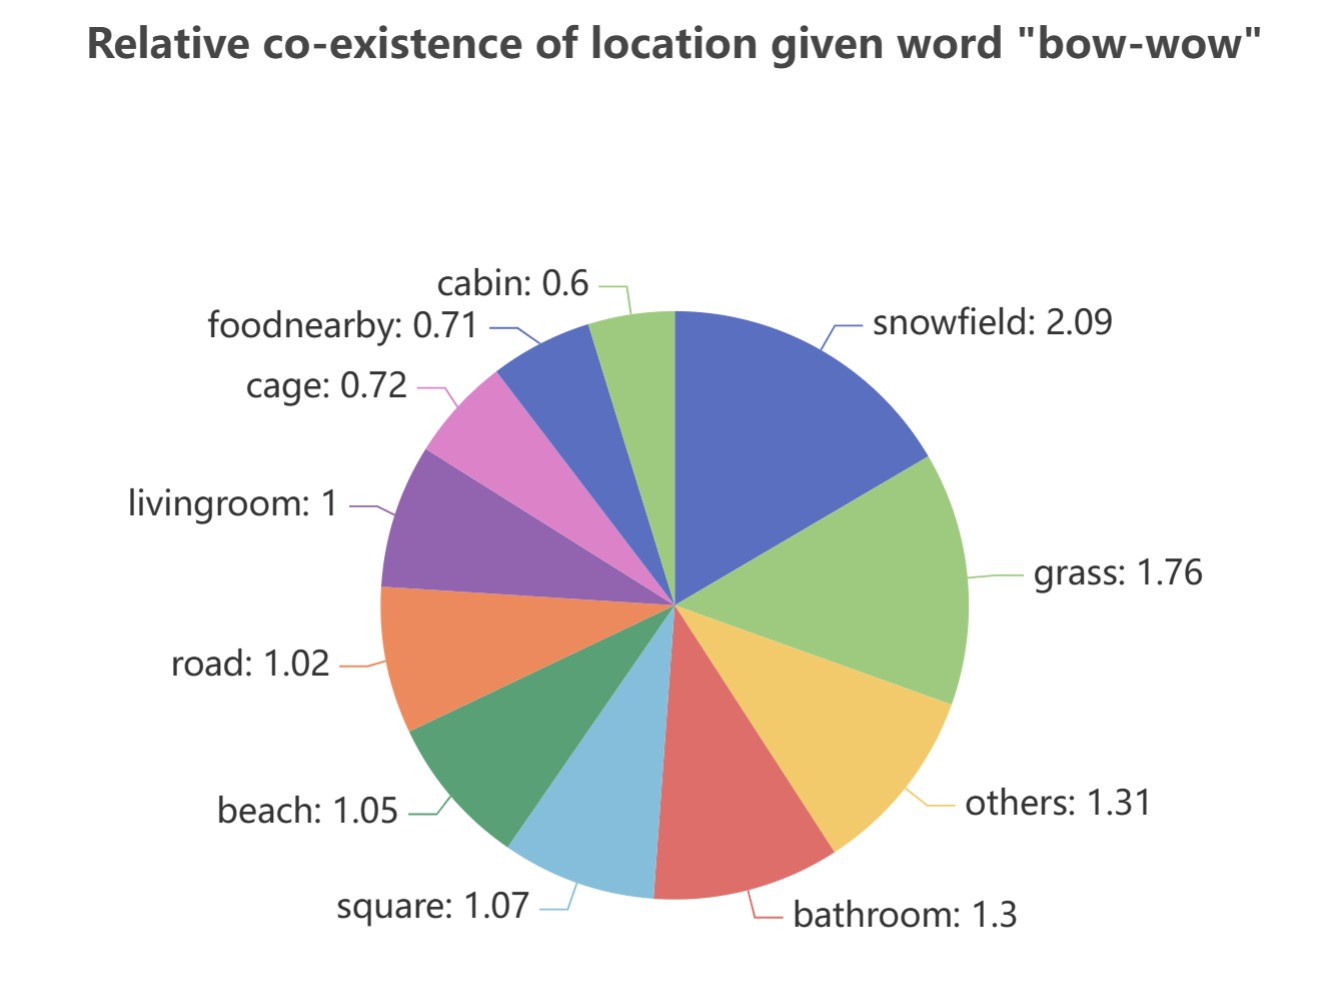
\includegraphics[width=0.8\columnwidth]{images/relative_bowwow.jpg}
	\caption{
%\KZ{There's actually no such thing called: The relative probability.} 
The probability of location given word ``bow-wow'' divided by location prior probability.}
	\label{fig:relative_bowwow}
\end{figure}

%\MY{For all these results, you should refer to specific numbers/comparisons from the probability, otherwise your readers cannot correspond the interpretations with the results}
%\AT{I explain in each item at which context it tends to do so}

Our analysis reveals several patterns between dog word types and 
corresponding locations with a minimum support number of 100 occurrences: 

%\KZ{Replace all uncomfort with discomfort.} 
%\KZ{When you make the following conclusions, what are min supports for each of these observations? 100, 10?}
%\AT{each item presents at least 100 times and each combinations are selected one shown more than 10 times.}
\begin{figure*}[th]
\centering
\begin{subfigure}[t]{0.49\textwidth}
	\centering
	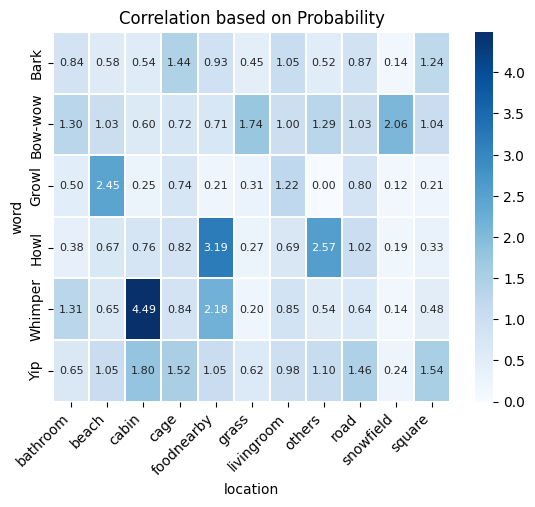
\includegraphics[width=0.9\textwidth]{images/sound_location_prior.png}
	\caption{Correlation between word types and locations.}
%\KZ{If you don't present the formula for each
%of these metrics, we don't even know how you come up with the numbers in
%these matrixes! This is unacceptable!}}
	\label{fig:sound_location}
\end{subfigure}
\begin{subfigure}[t]{0.49\textwidth}
	\centering
	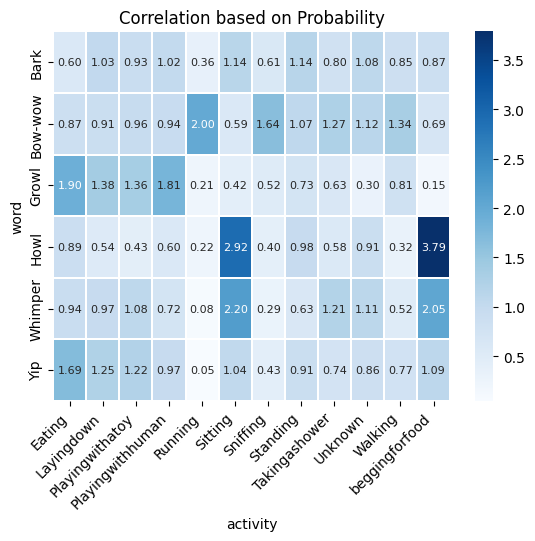
\includegraphics[width=0.9\textwidth]{images/sound_activity_prior.png}
	\caption{Correlation between word types and activities.}
	\label{fig:sound_activity}
\end{subfigure}

\begin{subfigure}[t]{0.49\textwidth}
	\centering
	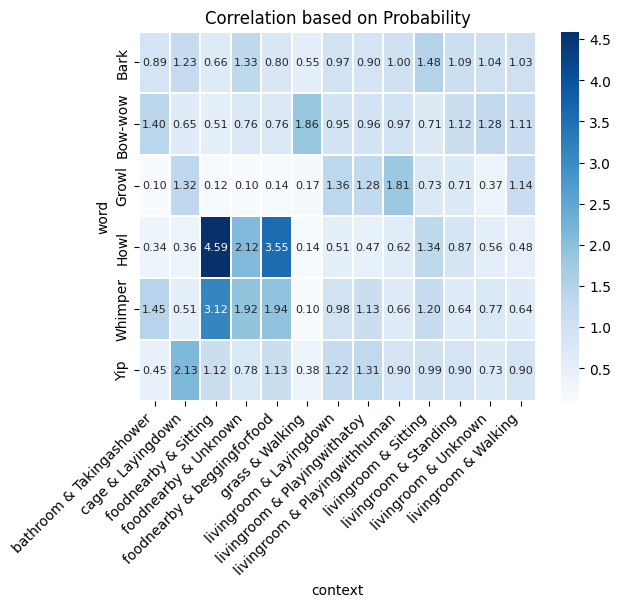
\includegraphics[width=0.9\textwidth]{images/one_sound_context.png}
	\caption{Correlation between word types and context.}
\label{fig:one_sound_context}
\end{subfigure}
\begin{subfigure}[t]{0.49\textwidth}
	\centering
	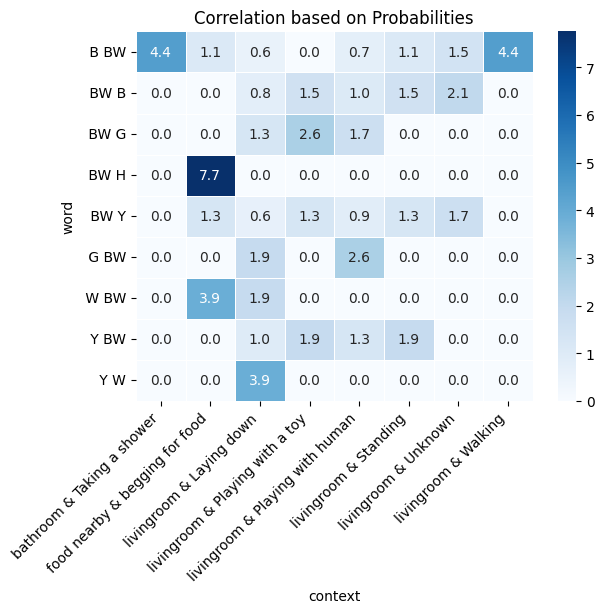
\includegraphics[width=0.9\textwidth]{images/sound_context_distri.png}
	\caption{Correlation between bi-gram and context. 
``B'', ``BW'', ``G'', ``H'', ``Y'', ``W'' represent ``bark'', ``bow-wow'', ``growl'', ``howl'', ``yip'' and ``whimper'' respectively.}
	\label{fig:sequenc_sound_context}
%\MY{y axis is sound, make sure that you are consistent in using word/sound to represent processed word types}}
%\KZ{There's both bow-wow growling and growling wow here. And their correlated
%contexts are a bit different. This is interesting. Because when you have AB
%and BA in this table, people might think that they were extracted from a seq
%like ABABA, and this seq should correspond to the same context. But it's not.
%So you should explain.}\AT{Hard to interpret it}}
\end{subfigure}
\caption{Correlation between lexical units and contexts.}
\label{fig:correlation}
\end{figure*}


\paragraph{``Bow-wow'' can be used to express curiosity.}
Bow-wows are usually used when they are outside and in unfamiliar surroundings like snowfields, grass, and beach as shown in \figref{fig:relative_bowwow}. This word may implicate an exploration of the environment. An example of ``bow-wow'' in snowfields is given in ~\figref{fig:bow-wow_snowfield}.


%\KZ{Do not repeat what is already bolded as headline.}

\paragraph{``Bark'' can be used to show anger and warning.} Bark, a more abrupt sound compared with ``bow-wow'', conveys many semantics and one of them is to express its anger and warning ~\cite{yeon2007vocal}. When the dog is located in a cage, it tends to ``bark'' as shown in Appendix ~\figref{fig:bark_cage}.


\paragraph{``Whimper'' can be seen as attention-seeking and a sign of 
discomfort.}
``Whimper'' can be used to show discomfort ~\cite{web2018dog} as dog whimpers when it is located in the bathroom when it is likely to take a shower or in a cage.
``Whimper'' can be used to elicit people attention ~\cite{handelman2012canine}. When there is food nearby, there may beg for food as shown in Appendix ~\figref{fig:whimper_attention}, and when in a cabin, it may want to interact with its host. 


\subsection{Analysis of word type and activity}
We use the same method to analyze the relationship between word types and 
activities: 
\begin{equation}
\frac{P (\text{activity}| \text{word})}{P(\text{activity})}
\end{equation}

From \figref{fig:sound_activity}, we have several observations:
%\KZ{$P(act | word)$}
\paragraph{``Bow-wow'' indicates movements.} Dogs exhibit a preference for using the ``bow-wow'' sound when engaging in activities that involve movement, such as walking, running, and sniffing. These actions are usually happened outside, which is coherent with our analysis of ``bow-wow'' and location. An example of ``bow-wow'' in movements is given in ~\figref{fig:bow-wow_walking}.

\paragraph{``Growl'' expresses playing interation.}
``Growl'' appears to be used to express positive playing interaction ~\cite{handelman2012canine}. It is also prevalent during eating because the dog wants to express its enjoyment. This kind of enjoyment is more than interaction. An example is given in ~\figref{fig:growl_play}.


\paragraph{``Howl'' can be seen as a signal for food.}
We find that Shiba Inu tends to ``howl'' when they are begging for food which is a new observation. And they are usually howling when sitting down. An example of ``Howl'' for food is given in ~\figref{fig:howl_food}.




\paragraph{``Whimper'' seeks contacting with human.}
Dogs often ``whimper'' when engaged in activities like sitting and begging for food. It may indicate contact seeking and a kind of submission ~\cite{pongracz2010barking}. 




\subsection{Analysis of word type and context}
When putting location and activity together:
\begin{equation}
\frac{P (\text{(location, activity)}| \text{word})}{P(\text{(location, activity)})}
\end{equation}

Because of the numerous combination possibilities for context, we define a threshold value of 100, indicating that a particular combination is considered statistically significant only if it occurs more than 100 times.
%\KZ{Rephrase: we set a threshold number to be 100, which means if and only this combination occurs more than 100 times then we think this 
%is statistically important.} 
~\figref{fig:one_sound_context} depicts this 
relationship between word type and context.
%\KZ{\[P((loc, act) | word)\]}



\paragraph{``Howl'' and ``Whimper'' come up frequently with food.} ``Howl'' and ``Whimper'' are strongly associated with ``food nearby'' and can be interpretated as an attention for food.
\paragraph{``Yip'' is a signal of discomfort.}  ``Yip'' can express pain or loneliness ~\cite{yeon2007vocal,web2018yip}. When the dog is located in the cage and laying down, it tends to yip. An example is given in ~\figref{fig:yip_cage}.


%\item When the dog is located in the cage, as the cage is small, it has to sit down and it may feel anger and ``bark''. 
%\item ``Howl'' and ``whimper'' can be seen as a signal for food. We think these two sounds express imploration and begging.


\subsection{Analysis of the sequence of triples}
To analyze the sequence of triples, we first select the words from the same sentence whose word type changes. We hypothesize a sequence of different word type in the same context also have a specific meaning. We set a threshold number of 10. So we only select the most frequency combinations and see them as a possible pattern instead of accidence. We explore the formula that:
\begin{equation}
\frac{P (\text{(location, activity)}| (w_1;w_2))}{P(\text{(location, activity)})}
\end{equation}
while $(w_1;w_2)$ represents two consecutive words with different types,
which is defined as a \textit{bi-gram} here. We highlight several insights. 
As shown in ~\figref{fig:sequenc_sound_context}, we use the same 
analysis method presented before. 

We find two possible patterns that contain semantics for Shiba Inu. 
First, ``Bark Bow-wow'' might be a sequence of words to express discomfort as it is highly probable to take a shower in the bathroom, as this always makes the dog uncomfortable and angry. ``Bark'' and ``bow-wow'' are both words that can convey many meanings~\cite{yeon2007vocal} and the main different between them is the pitch.
Second, ``Bow-wow Howl'' and ``Whimper Bow-wow'' can be seen as a signal for asking for food as shown in ~\figref{fig:Whimper_Bow-wow_food}. This corresponds with our previous analysis. 
%\KZ{\[P ((loc, act) | (w_1; w_2)) \]}

%\item Normally, a combination of ``BA'' may have a similar distribution of probability of ``AB'', as they all may come from a sequence like ``ABABA''. But here, our data distribution of ours is unlike this. It may be because the order of the sounds is also part of its semantics. 




\subsection{Analysis of bi-gram probability}
In this section, we analyze the bi-gram probability for two-word sequences 
as $w_1$ followed by $w_2$, where $w_1$ and $w_2$ represent two words. 
To facilitate the comprehension, we further divide each item by $w_2$ 
prior distribution to show relative changes. The result for: 
%To facilitate the comprehension, we further divide each item by $w_2$ 
%prior distribution to show relative changes. 
\begin{equation}
{P (w_1|w_2)}
\end{equation}
is shown in Appendix ~\figref{tab:bigramword}. 

We make two observations here. First, ``Bark'' and ``bow-wow'' show a 
similar distribution of relative probability and may share similar semantics. 
``Whimper'' and ``Yip'' may also 
convey the same semantics for similar distribution. Second, for ``growl'' 
and ``howl'', they are always followed by the same word, 
implying that these words each contain a special meaning. The subtle difference between these words can be further studied. 


%\KZ{I think something can be said such as:
%BW often follows B, but B doesn't follow BW as much. BW also follows G, but
%no so much after H, many words can follow W, and after a Y, there's always a
%BW. Some of the these bigrams we have meanings, others we don't. But at least
%we know these are the popular patterns for future study?}
%\AT{This is because we do not divide them by prior probability, which is asked not to do so.}

%\KZ{I think something can be said such as:
%BW often follows B, but B doesn't follow BW as much. BW also follows G, but
%no so much after H, many words can follow W, and after a Y, there's always a
%BW. Some of the these bigrams we have meanings, others we don't. But at least
%we know these are the popular patterns for future study?}
%\AT{This is because we do not divide them by prior probability so we have such feeling, which is asked not to do so. }

    



\subsection{Comparison with Previous Works}
%\KZ{At the end of this, we can have a table that summarizes all the 
%interesting findings: word/bigram, the meaning we discovered, its previously
%known meaning, citation of prev meanings.}
In this section, We present our findings including the evidence to support previous theoretical studies and our new observations.
Through the analysis, we found most of the patterns we mentioned are consistent with the previous qualitative research. We also discover more detailed interpretations of those existing patterns and provide possible new findings.

%\MY{u discover more detailed interpretations of those existing patterns, and provide possible new findings. then give examples, possibly using the bi-gram results as previously no one does this }
%\AT{if doing so, it may be redundant as i explained in each item which words have new meaning and which are consistent with existing research}

A brief summarization can be seen in \tabref{tab:finding}. 
``Bow-wow'' can be seen as a low-pitch ``bark'' and previous work like conflating them. Our findings suggest ``bow-wow'' and ``bark'' have a lot in common, but ``bow-wow'' has its own unique meaning, dissimilar to ``bark''. 

%\begin{table}[th]
%\small
%\begin{tabular}{p{0.2\columnwidth}|p{0.7\columnwidth}}

%\toprule
%\textbf{Findings} & \textbf{Explanation} \\ \midrule
%Conformity & 
%\makecell[l]{1.``Bark'' can show the anger and warning. \\
%2.``Growl'' expresses playing interaction.\\
%3.``Whimper'' can be seen as attention-\\seeking and a sign of discomfort. \\
%4.``Yip'' is a signal of discomfort.}
% \\ \midrule
%New observations & 
%\makecell[l]{
%1.``Bow-wow'' can be used to express \\curiosity and it is usually seen when \\dog is in movement.\\
%2.``Bark Bow-wow'' are highly used when \\dog is forced. \\
%3.``Bow-wow Howl'' and ``Whimper Bow-\\wow'' are usually used for asking food.}
% \\ 
%\bottomrule
%\end{tabular}
%\caption{Overall findings of the analysis.}
%\label{tab:findings}
%\end{table}

%\KZ{Maybe try this to summarize the findings in comparison with the
%previous studies?}
%\AT{new findgins means that we find something that never mentioned before, but we do not show contradictions with previous work}

\begin{table*}[th]
\small
\centering
\begin{tabular}{p{0.6\columnwidth}|p{0.6\columnwidth}|p{0.6\columnwidth}}
\toprule
\textbf{Lexical Symbols} & \textbf{Previous Meaning} & \textbf{Our Meaning}\\
\hline
Whimper & attention-seeking \cite{handelman2012canine},
				discomfort \cite{web2018dog} & attention-seeking,discomfort \\
\hline
Yip & discomfort ~\cite{web2018yip} & discomfort \\
\hline
Bow-wow & NA & show curiosity, movement\\
\hline
Growl & playing interaction ~\cite{handelman2012canine} & playing interation, enjoyment \\
\hline
Bark & warning \cite{handelman2012canine} & anger \\
\hline
Howl & warning, play, group cohesion ~\cite{ani8080131} & signal for food \\
\hline
Bark Bow-wow & NA & discomfort \\
\hline
Bow-wow Howl & NA & signal for food \\
\hline
Whimper Bow-wow & NA & signal for food \\
\bottomrule
\end{tabular}
\caption{Summary of findings with comparison to previously-discovered meanings.}
%\KZ{Caption is either on the top
%or on the bottom. Be consistent. Make this table a narrow one. Use
%acronyms to save space.}}
\label{tab:finding}
\end{table*}




%People believe:
%\begin{itemize}
%\item Bark: short-range interaction; high pitch are made in isolation situation, stranger; 
%\item Growl: agonistic interactions as a warning or threatening signal or during play interactions. 
%\item whine: indicators of stressful arousal but also greeting and attention-seeking behaviours
%\item howls, which maintain group cohesion
%\item groans and yelps, signs of acute distress and acute pain, respectively; and grunts, which are considered as pleasure-related signals
%\item They mainly use short-distance calls in interactions with humans, like barks, growls, and whines, compared with long distance calls, which are used instead to communicate with conspecifics
%\end{itemize}

%Conformity:
%the difference between bow-wow and bark: mainly frequence

%\begin{itemize}
%\item Whimper sttention-seeking cabin, food, cage
%\item Bark anger, high pitch are made in isolation situation(located in a room isolated from its owner) like in cage
%\item growling: play interaction
%\item howl draw attention for begging for food
%\item bark bow-wow when bathing, discomfort
%\end{itemize}

%Our new finding:
%\begin{itemize}
%\item Bow-wow can be used to show dog exploring the outside world or curiosity;
%\item Growling may also show enjoyment when the dog is laying down and eating;
%\item Dogs like to bow-wow when moving around; and like to howl, whimper, or 
%yip when they are stationary.
%\end{itemize}
